\begin{frame}[t]{¡A practicar!}

    \begin{ejercicio}{Ejercicio de a 2 máquinas (preferiblemente 2 personas): \emoji{christmas-tree} y \emoji{jack-o-lantern}}
        \begin{enumerate}\begin{small}
            \pause
        \item \emoji{christmas-tree}: crear un repositorio nuevo en \href{https://git.cubawiki.com.ar}{Forgejo}, tildando la opción \textit{Inicializar el repositorio}. Una vez creado, en la configuración del repositorio agregar a \emoji{jack-o-lantern} como colaborador.
            \pause
            \item \emoji{christmas-tree} y \emoji{jack-o-lantern}: obtener una copia local del repo usando \texttt{git clone <URL>}.

            \pause
            \item \emoji{christmas-tree}:
            crear un archivo \textit{navidad.txt} con unas palabras acerca de la navidad.
            \item \emoji{jack-o-lantern}: crear un archivo \textit{halloween.txt} con unas palabras acerca de halloween.
            \pause
            \item \emoji{christmas-tree} y \emoji{jack-o-lantern}: hagan \textit{commits} con sus cambios respectivos.
            \pause
            \item \emoji{christmas-tree}: hacer \texttt{git push} con sus cambios.
            \pause
            \item \emoji{jack-o-lantern}: intentar hacer \texttt{git push} de los cambios al repo remoto. ¿Qué pasó?
            \pause
        \item \emoji{jack-o-lantern}: bajarse los cambios del repositorio remoto. con \texttt{git pull --no-rebase}. ¿Anduvo?
            \pause
            \item \emoji{jack-o-lantern}: \textit{pushear} el resultado.
            \pause
            \item \emoji{christmas-tree}: bajarse los nuevos cambios.
        \end{small}\end{enumerate}
    \end{ejercicio}

\end{frame}

\begin{frame}{Visualizando los cambios 1/2}
\begin{center}
    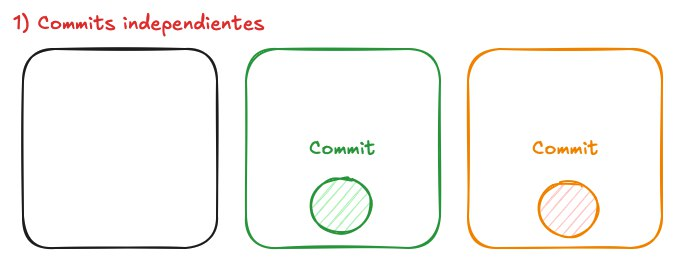
\includegraphics[width=2.5in]{images/merge1.jpg}
    \pause
    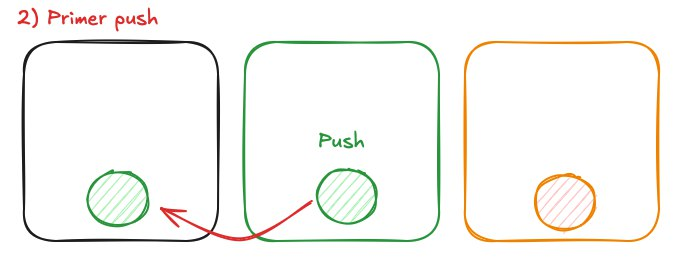
\includegraphics[width=2.5in]{images/merge2.jpg}
    \pause
    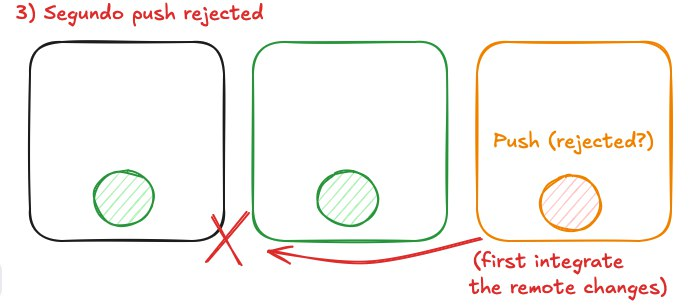
\includegraphics[width=2.5in]{images/merge3.jpg}
\end{center}
\end{frame}

\begin{frame}{Visualizando los cambios 2/2}
\begin{center}
    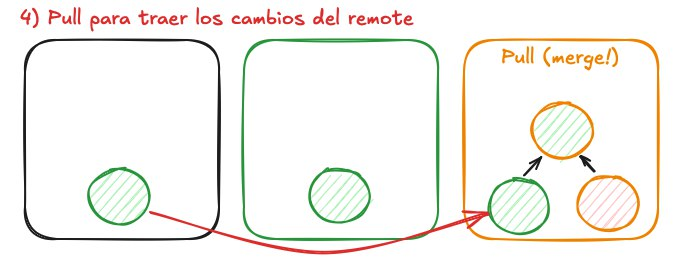
\includegraphics[width=2.5in]{images/merge4.jpg}
    \pause
    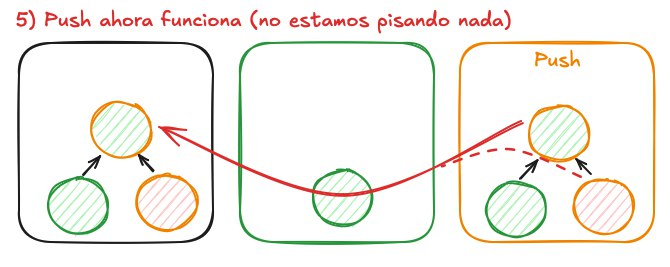
\includegraphics[width=2.5in]{images/merge5.jpg}
    \pause
    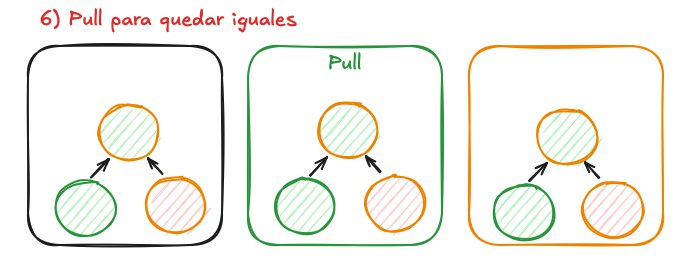
\includegraphics[width=2.5in]{images/merge6.jpg}
\end{center}

\end{frame}

